\documentclass[Thesis.tex]{subfiles}
\begin{document}

\chapter{Discrete Uniformization}
\label{chp:uniformization}

\section{Map to the disk}
\label{sec:disk_mapping}

\section{Multiply-connected regions}
\label{sec:multiply_connected_regions}

\section{Quotient spaces and fundamental domains}
\label{sec:fundamental_domains}

Every Riemann surface $R$ has a universal cover $X$, i.e., a simply connected covering space and a corresponding covering map. A metric of constant curvature on a compact $2$-manifold can be realized as the quotient of the universal cover over a uniformizing group.

Triangulated surfaces of genus $g\geq 2$ without boundary can be equipped with a discretely conformally equivalent flat hyperbolic metric \cite{Bobenko2010}. By flat hyperbolic metric we mean that the edge length are hyperbolic and for any vertex the angle sum is $2\pi$. To realize this metric in the hyperbolic plane e.g. in the Poicar\'e disk model one has to introduce cuts along a basis of the homotopy. This creates a simply connected domain in $\mathbb H^2$. Matching cut paths are realated by a hyperbolic motion i.e. the M\"obius transformations that leave the unit disk invariant (Figure~\ref{fig:axes_of_motion}).

\subsection{The cut-graph and fuchsian groups}
\emph{Want so say here: the number of transformations generated by the mapping of corresponding edges equals the number of path segments in the homotopy-cut-graph. They generate a fuchsian group with \#vertices relations}


\begin{figure}
\centering
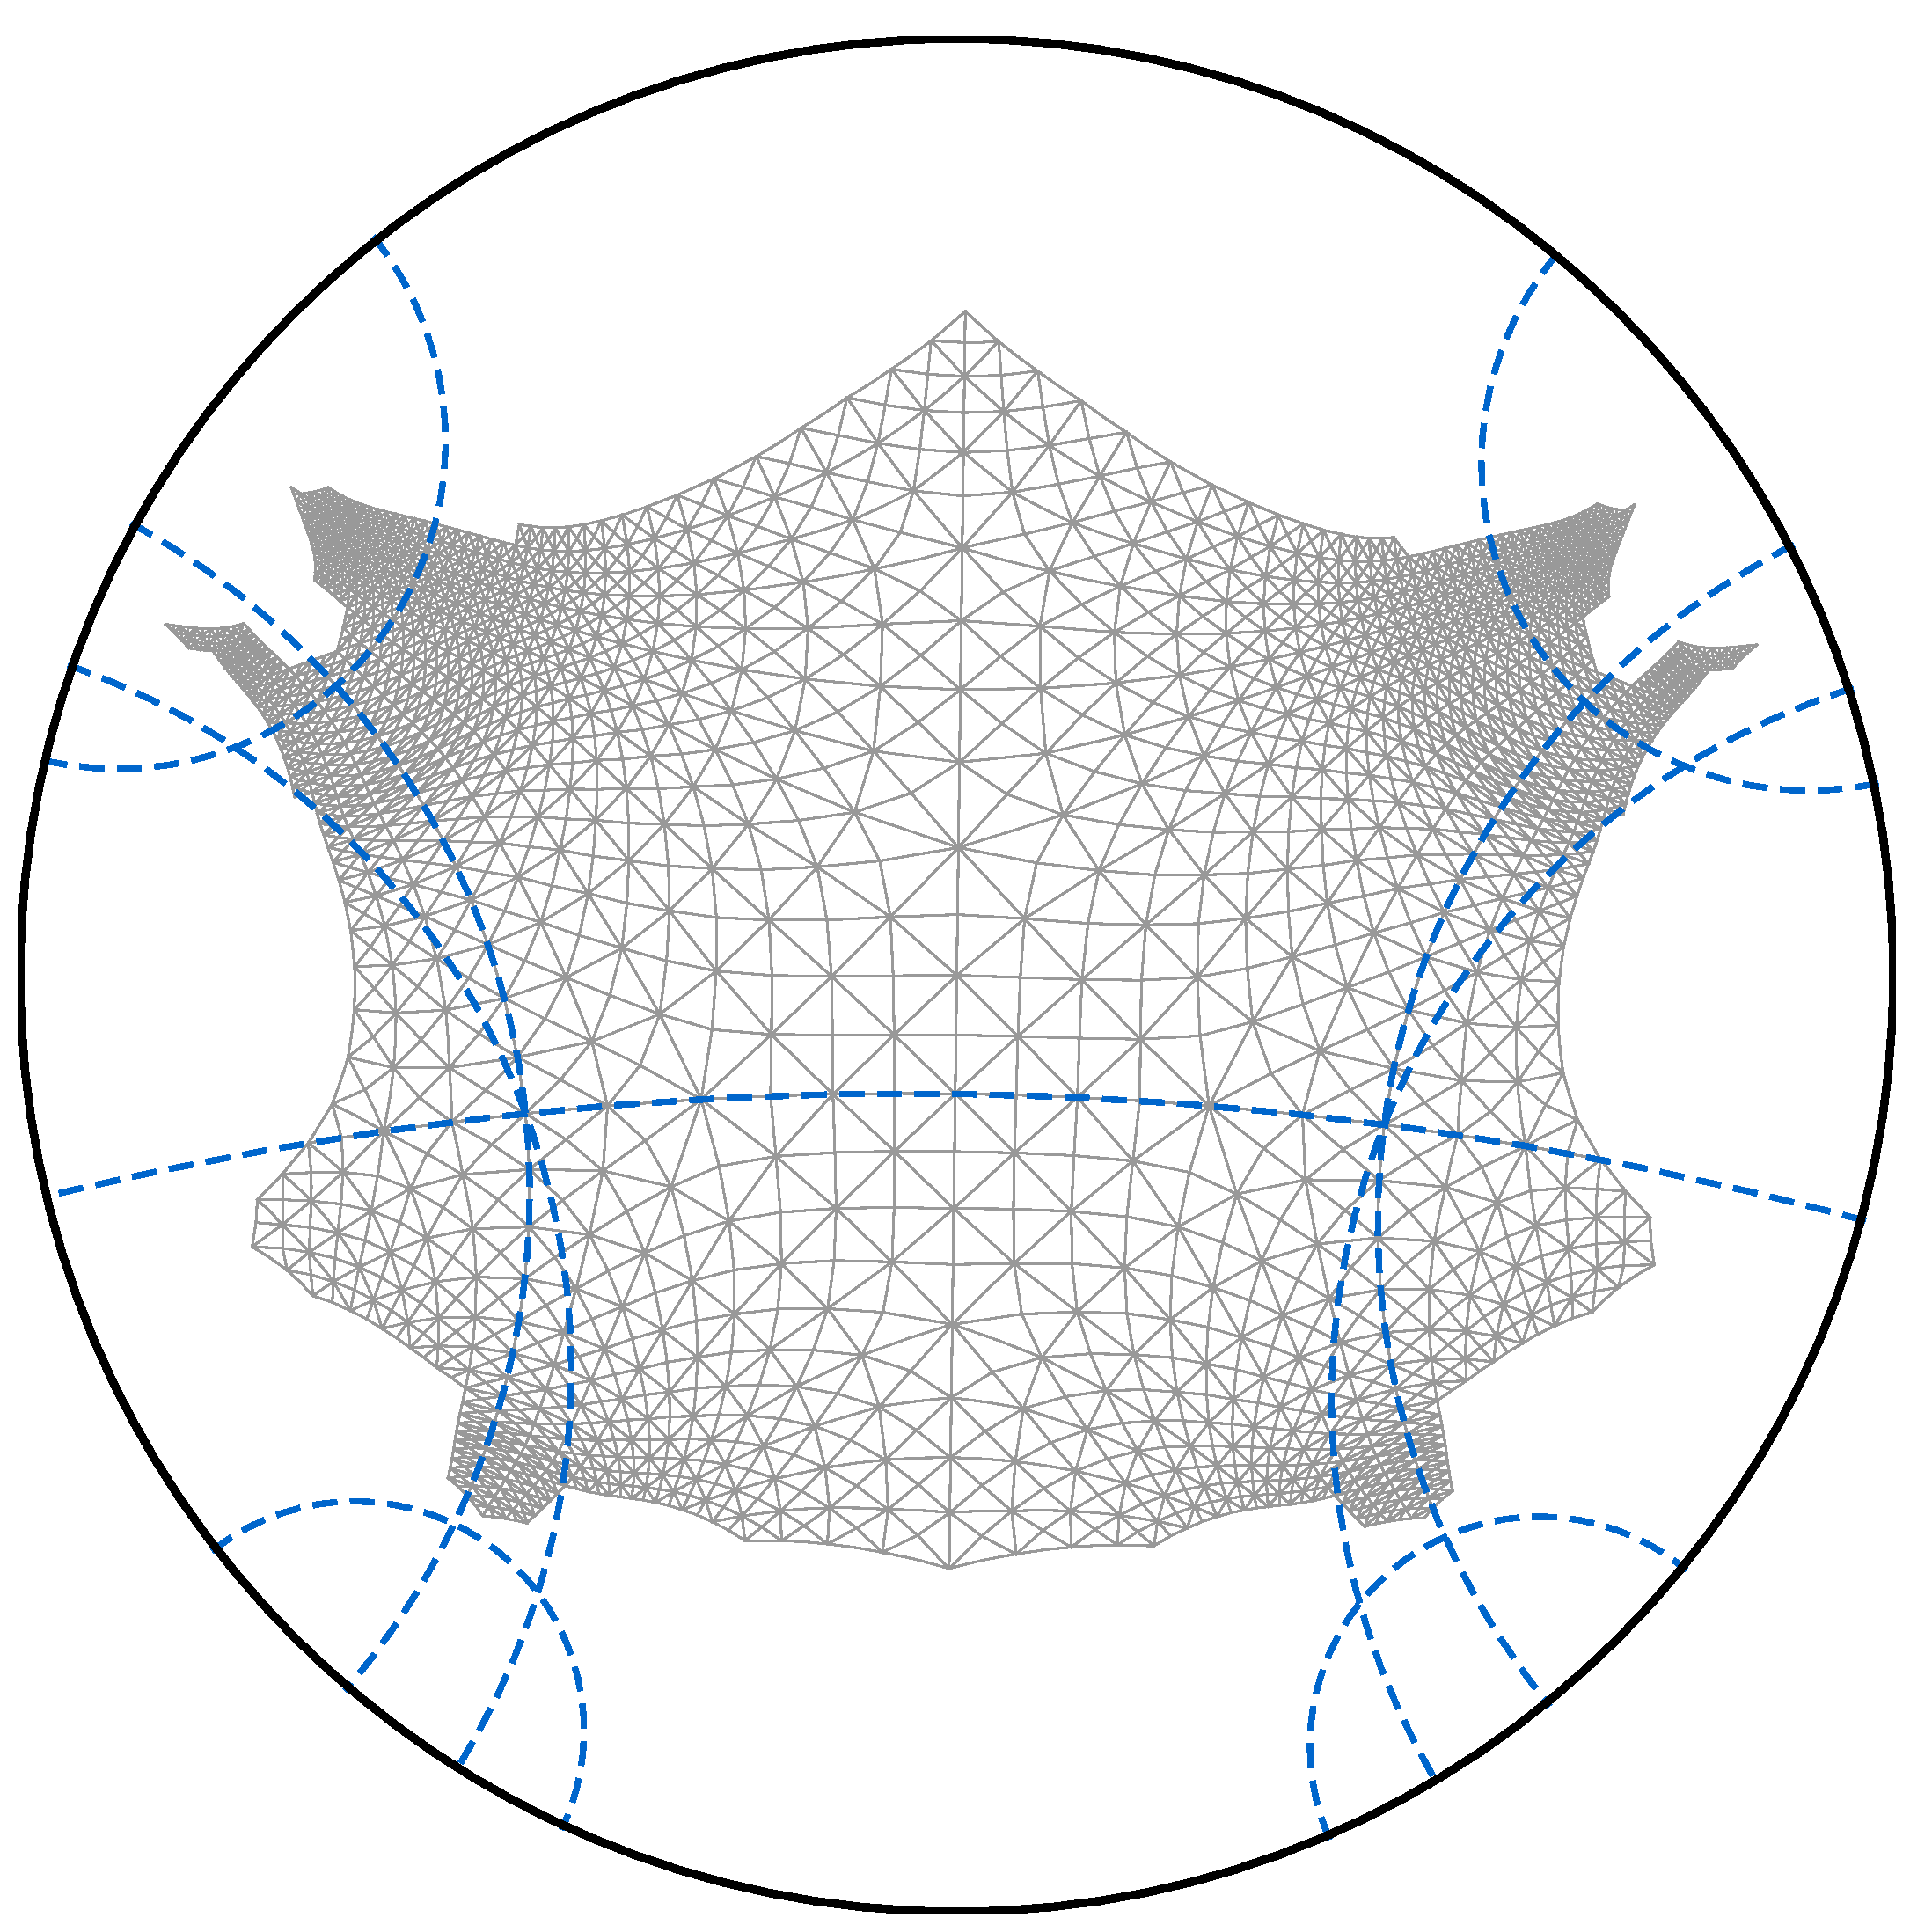
\includegraphics[width=0.4\linewidth]{cutCuttedBrezel01}
\caption{Hyperbolic flat metric on a genus $2$ surface and the axes of the associated hyperbolic motions.}
\label{fig:axes_of_motion}
\end{figure}

\subsection{Minimal presentation}
\subsection{Separated handles}
\subsection{Opposite sides identified}
\subsection{Canonical Keen Polygons}

\section{Uniformization of embedded genus $g=0$, $g=1$, and $g>1$ surfaces}

\begin{figure}

\caption{Lawson's surface}
\end{figure}

\subfilebibliography
\end{document}

%%% Local Variables:
%%% TeX-master: "Thesis.tex"
%%% End: